\chapter[KAJIAN PUSTAKA]{Kajian Pustaka}
\label{chap:kajian-pustaka}

Bab ini membahas konsep yang menjadi landasan konseptual bagi kajian RAG modular. Uraian mencakup pembentukan unit dokumen, pengindeksan, \emph{knowledge graph}, pengelolaan konteks percakapan, perlindungan PII, \emph{guardrail}, dan evaluasi. Akuisisi dokumen, \emph{scraper}, ekstraksi PDF, dan OCR tidak dibahas karena berada di luar ruang lingkup kajian ini.

\section{Model Bahasa Besar dan Kebutuhan akan Sumber Eksternal}

LLM modern umumnya dibangun menggunakan arsitektur \emph{Transformer}. Arsitektur ini memanfaatkan \emph{self-attention} untuk memodelkan hubungan antartoken tanpa memproses urutan secara rekuren \parencite{vaswaniAttentionAllYou2023}. Setelah menjalani pelatihan awal dan penyelarasan instruksi, model dapat digunakan untuk menjawab pertanyaan, merangkum teks, dan menghasilkan keluaran terstruktur.

Pengetahuan yang digunakan LLM tersimpan secara parametris. Bentuk penyimpanan ini memungkinkan model menghasilkan teks tanpa mengakses basis data pada setiap permintaan, tetapi mempunyai beberapa keterbatasan. Sumber sebuah pernyataan tidak selalu dapat ditunjukkan, pembaruan informasi membutuhkan proses tambahan, dan model dapat menghasilkan isi yang tidak didukung oleh fakta. Ji dkk. membedakan halusinasi yang bertentangan dengan sumber masukan dari halusinasi yang tidak dapat diverifikasi terhadap pengetahuan faktual \parencite{jiSurveyHallucinationNatural2023}.

Memperbesar jendela konteks juga tidak serta-merta menyelesaikan persoalan tersebut. Liu dkk. menemukan bahwa kinerja model dapat menurun ketika informasi yang relevan berada di bagian tengah konteks panjang, sebuah gejala yang dikenal sebagai \emph{lost in the middle} \parencite{liuLostMiddle2024}. Temuan tersebut menunjukkan bahwa pemilihan dan penempatan informasi tetap penting, bahkan ketika model mampu menerima masukan yang panjang.

Dalam sistem berbasis sumber eksternal, konsep \emph{grounding} digunakan untuk mengikat jawaban pada informasi yang dapat diperiksa. LLM tetap berperan dalam memahami pertanyaan dan membentuk penjelasan, sedangkan fakta utama berasal dari dokumen atau struktur pengetahuan yang mempunyai identitas sumber. Dengan cara ini, kelancaran bahasa dipisahkan dari otoritas bukti.

\section{\emph{Retrieval-Augmented Generation}}

RAG menggabungkan memori parametris pada model bahasa dengan memori nonparametris berupa koleksi eksternal \parencite{lewisRetrievalAugmentedGenerationKnowledgeIntensive2021}. Jika $q$ menyatakan pertanyaan, $D$ koleksi dokumen, $R_k$ fungsi pencarian yang menghasilkan $k$ konteks berperingkat, dan $G$ generator, prosesnya dapat disederhanakan menjadi:

\begin{equation}
    y = G\bigl(q,R_k(q,D)\bigr).
\end{equation}

Persamaan tersebut memperlihatkan hubungan dasar antara pencarian dan generasi, tetapi RAG dalam penerapan nyata mempunyai tahapan yang lebih luas. Dokumen perlu disiapkan dan diindeks sebelum dapat dicari. Kueri dapat diubah sebelum pencarian, hasil dapat disaring atau diurutkan ulang, dan konteks terpilih perlu disusun sebelum diberikan kepada \emph{generator}.

\begin{figure}[htbp]
    \centering
    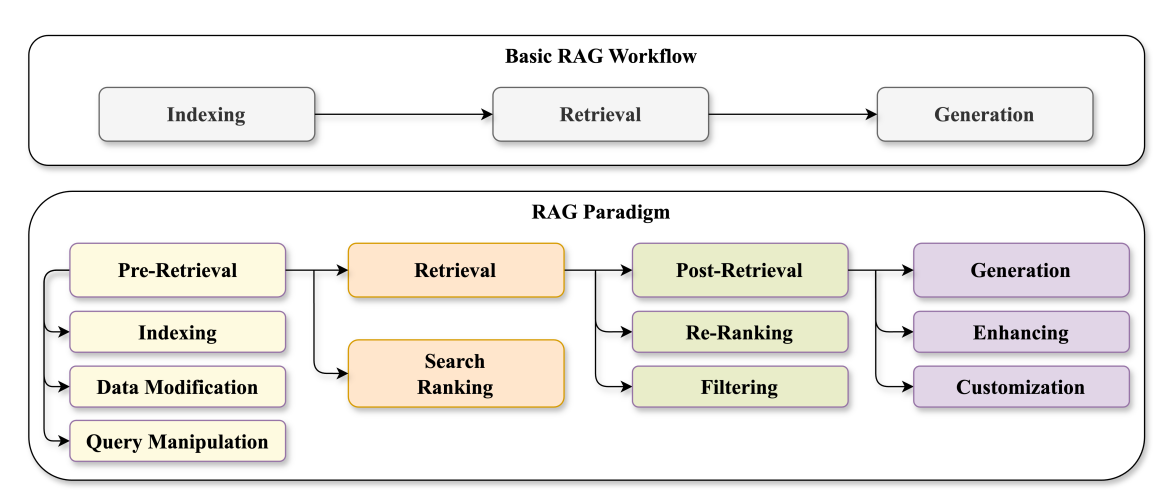
\includegraphics[width=0.96\textwidth]{images/reference-002.png}
    \caption{Tahapan umum pada RAG, mulai dari pemrosesan sebelum pencarian hingga generasi (sumber: \textcite{huangSurveyRetrievalAugmentedText2024})}
    \label{fig:rag-paradigm-literature}
\end{figure}

Gambar \ref{fig:rag-paradigm-literature} memperlihatkan bahwa RAG tidak terbatas pada pola ``cari lalu jawab''. Huang dan Huang mengelompokkan proses menjadi tahap sebelum pencarian, pencarian, sesudah pencarian, dan generasi \parencite{huangSurveyRetrievalAugmentedText2024}. Tahap sebelum pencarian dapat mencakup pengindeksan, modifikasi data, dan manipulasi kueri. Tahap sesudah pencarian dapat mencakup \emph{reranking} serta penyaringan sebelum konteks diberikan kepada model.

\subsection{\emph{Modular RAG}}

RAG awal sering digambarkan sebagai alur linear. Ketika kebutuhan aplikasi berkembang, sistem dapat menggunakan lebih dari satu pencari, memilih strategi berdasarkan kueri, mengulang pencarian, atau menggabungkan beberapa jenis sumber. Gao dkk. memperkenalkan kerangka \emph{Modular RAG} dengan memisahkan proses menjadi modul dan operator \parencite{gaoModularRAG2024}. Kerangka tersebut mencakup pola linear, bersyarat, bercabang, dan berulang.

Kontribusi utama \emph{Modular RAG} terletak pada cara melihat RAG sebagai komposisi kemampuan, bukan satu rangkaian yang tidak dapat diubah. Pemisahan ini memudahkan penggunaan \emph{routing}, \emph{scheduling}, dan fusi pada titik yang berbeda. Namun, kerangka konseptual tersebut tidak menentukan satu bentuk kontrak perangkat lunak. Skema data, versi komponen, aturan kompatibilitas, dan pencatatan \emph{artifact} tetap menjadi keputusan setiap implementasi.

\section{Arsitektur \emph{Pipeline}, \emph{Plugin}, dan Representasi Kanonik}

Arsitektur \emph{pipeline} memandang pemrosesan sebagai rangkaian komponen yang menerima masukan, melakukan satu tanggung jawab utama, lalu menghasilkan keluaran untuk komponen berikutnya. Pada gaya \emph{pipes and filters}, setiap \emph{filter} tidak perlu mengetahui cara kerja komponen lain selama bentuk data di antara keduanya dipertahankan \parencite{garlanIntroductionSoftware1994}. Pemisahan ini penting pada sistem dokumen karena perubahan cara memperoleh atau membaca dokumen tidak seharusnya memaksa perubahan pada pencarian dan generasi.

\emph{Plugin} memberikan titik perluasan bagi variasi yang memang tidak dapat digeneralisasi. Sebuah \emph{plugin} biasanya membawa identitas, versi, titik masuk, konfigurasi, dan kontrak keluaran. Registri atau katalog kemudian memilih implementasi berdasarkan identitas tersebut. Keuntungan utamanya adalah penambahan sumber atau strategi baru dapat dilakukan tanpa menanamkan percabangan khusus ke dalam orkestrator. Namun, \emph{plugin} hanya dapat dipertukarkan jika skema data, kemampuan keluaran, dan aturan kompatibilitasnya dinyatakan secara eksplisit.

Pada pemrosesan dokumen, kontrak antartahap sering diwujudkan sebagai representasi kanonik. Representasi ini mempertahankan identitas dokumen, teks, struktur, lokasi, \emph{metadata}, dan asal pembentuknya dalam bentuk yang sama untuk semua jalur. Dokumen kanonik berperan sebagai batas yang memisahkan cara membaca sumber dari cara membentuk unit pencarian. Dengan batas tersebut, komponen hilir tidak perlu mengetahui format atau mekanisme sumber yang menghasilkan teks.

\section{\emph{Document Chunking}}

\emph{Document chunking} membagi dokumen menjadi unit yang akan dicari. Batas unit menentukan informasi apa yang dinilai sebagai satu kesatuan. Potongan yang terlalu besar dapat membawa konteks lengkap, tetapi menambahkan bagian yang tidak relevan. Potongan yang terlalu kecil meningkatkan ketepatan lokasi, tetapi dapat memisahkan subjek, syarat, atau pengecualian dari isi yang dijelaskannya.

Untuk dokumen $d$ dengan panjang $L$, fungsi \emph{chunking} dapat ditulis sebagai:

\begin{equation}
    C(d\mid\theta)=\{c_1,c_2,\ldots,c_n\},
\end{equation}

dengan $\theta$ memuat metode, satuan ukuran, batas panjang, dan kebijakan \emph{overlap}. Parameter yang sama tidak selalu mempunyai arti yang sama pada metode berbeda. Ukuran pada \emph{sliding window} menyatakan panjang irisan, sedangkan ukuran pada \emph{recursive chunking} menjadi batas setelah pemisah alami dicoba.

\subsection{\emph{Sliding Window}}

\emph{Sliding window} memotong urutan dengan panjang tetap $w$ dan \emph{overlap} $o$. Jendela berikutnya dimulai setelah pergeseran $w-o$. Jika $t_1,\ldots,t_L$ menyatakan unit teks, potongan ke-$i$ dapat ditulis sebagai:

\begin{equation}
    c_i=t_{1+(i-1)(w-o)}\ldots t_{w+(i-1)(w-o)}.
\end{equation}

Metode ini deterministik, murah, dan mudah digunakan sebagai \emph{baseline}. \emph{Overlap} membantu mengurangi kehilangan informasi pada batas potongan, tetapi meningkatkan duplikasi dan ukuran indeks. Karena batasnya tidak memahami struktur teks, judul dapat terpisah dari isi dan ketentuan dapat terpisah dari pengecualiannya.

\subsection{\emph{Recursive Chunking}}

\emph{Recursive chunking} mencoba pemisah dari batas yang lebih kuat menuju batas yang lebih lemah, misalnya paragraf, baris, kalimat, spasi, lalu pemisahan keras. Sebuah bagian hanya dipecah lagi ketika panjangnya masih melampaui batas. Cara ini berusaha mempertahankan bentuk alami teks tanpa memerlukan model semantik untuk setiap dokumen.

Keunggulan pendekatan rekursif adalah kompromi antara kesederhanaan dan koherensi. Paragraf yang pendek dapat dipertahankan sebagai satu unit, sedangkan bagian panjang tetap mempunyai \emph{fallback}. Kinerjanya tetap dipengaruhi oleh kualitas pemisah dan karakteristik dokumen. Narimissa dan Raithel menunjukkan bahwa metode pemisahan serta karakteristik dokumen memengaruhi kualitas pencarian, sehingga nilai ukuran dan \emph{overlap} tidak dapat dianggap universal \parencite{narimissaExploringInformationRetrieval2024}.

\subsection{\emph{Structure-Aware Chunking}}

\emph{Structure-aware chunking} menggunakan struktur dokumen sebagai batas awal. Judul, subjudul, paragraf, daftar, atau unit hasil penguraian dipertahankan bersama jalur hierarkinya. Pendekatan ini berguna ketika makna sebuah paragraf bergantung pada judul di atasnya. AutoChunker, misalnya, membentuk representasi pohon dan menggunakan model bahasa untuk memisahkan unit informasi sambil mengurangi \emph{noise} \parencite{jainAutoChunker2025}. Penelitian tersebut menilai potongan berdasarkan pengurangan \emph{noise}, kelengkapan, koherensi konteks, relevansi tugas, dan kinerja pencarian.

Untuk dokumen hukum, struktur bukan hanya persoalan tata letak. Penanda seperti Bagian, Bab, Pasal, Ayat, Huruf, dan Angka membentuk hierarki yang membantu menafsirkan kedudukan sebuah ketentuan. Oleh karena itu, potongan sebaiknya menyimpan jalur induk dan \emph{metadata} penanda, sementara teks anak tetap dibatasi agar pencarian tidak menghasilkan unit yang terlalu besar. NitiBench membandingkan pemotongan naif dengan pemotongan yang mempertahankan hierarki pada tanya jawab hukum Thailand \parencite{akarajaradwongNitiBenchComprehensiveStudy2025}. Ilustrasinya disajikan pada Gambar \ref{fig:nitibench-chunking-literature}.

\begin{figure}[htbp]
    \centering
    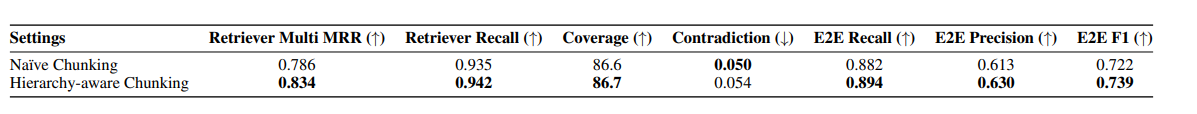
\includegraphics[width=0.94\textwidth]{images/reference-003.png}
    \caption{Perbandingan \emph{naive chunking} dan \emph{hierarchy-aware chunking} pada NitiBench (sumber: \textcite{akarajaradwongNitiBenchComprehensiveStudy2025})}
    \label{fig:nitibench-chunking-literature}
\end{figure}

Hasil NitiBench menunjukkan adanya perbaikan dari komponen khusus \emph{domain}, tetapi peningkatannya bersifat terbatas dan pencarian untuk pertanyaan hukum kompleks tetap sulit. Nilai tersebut juga tidak dapat dipindahkan langsung ke sistem hukum lain karena bahasa, bentuk peraturan, korpus, model, dan label bukti berbeda. Dengan demikian, \emph{structure-aware chunking} diperlakukan sebagai hipotesis desain yang perlu dibandingkan secara empiris, bukan sebagai metode yang selalu unggul.

\subsection{\emph{Parent--Child Chunking}}

Pada \emph{parent--child chunking}, pencarian dilakukan terhadap unit anak yang lebih kecil, sedangkan unit induk yang lebih lengkap dikembalikan sebagai konteks. Pola ini juga disebut \emph{small-to-large retrieval}. Tujuannya adalah mempertahankan ketepatan pencarian tanpa mengorbankan kelengkapan konteks yang dibaca model. Hubungan tersebut dapat ditulis sebagai pemetaan $p(c_i)=u_j$, dengan $c_i$ sebagai unit anak dan $u_j$ sebagai unit induk yang memuatnya.

Metode ini berbeda dari \emph{structure-aware chunking}. \emph{Structure-aware chunking} menentukan batas potongan berdasarkan struktur dokumen, sedangkan \emph{parent--child chunking} menentukan dua tingkat representasi untuk tujuan pencarian dan penyusunan konteks. Keduanya dapat dipakai bersamaan: struktur hukum membentuk induk dan anak, kemudian anak digunakan untuk pencarian sementara induknya digunakan untuk \emph{context hydration}. Risiko utamanya adalah duplikasi ketika banyak anak dari induk yang sama masuk dalam kandidat serta penambahan konteks yang melampaui anggaran \emph{token}. Karena itu, penggabungan induk perlu melakukan deduplikasi dan mempertahankan identitas sumber.

\section{Pengindeksan dan Pencarian Informasi}

Pengindeksan mengubah potongan dokumen menjadi representasi yang dapat dicari. Literatur pencarian informasi membedakan pendekatan leksikal, semantik, dan hibrida. Ketiganya tidak hanya berbeda pada teknologi penyimpanan, tetapi juga pada jenis kecocokan yang dianggap penting.

\subsection{Pencarian Leksikal}

Pencarian leksikal membandingkan istilah pada kueri dengan istilah pada dokumen. BM25 memberi bobot lebih besar pada istilah yang jarang dan menormalkan pengaruh panjang dokumen \parencite{robertsonProbabilisticRelevanceFramework2009}. Bentuk umum skornya adalah:

\begin{equation}
\operatorname{BM25}(q,d)=
\sum_{t\in q}\operatorname{IDF}(t)
\frac{f(t,d)(k_1+1)}
{f(t,d)+k_1\left(1-b+b\frac{|d|}{\operatorname{avgdl}}\right)}.
\end{equation}

Pencarian leksikal berguna ketika istilah perlu cocok secara tepat, misalnya kode galat, nama produk, nomor peraturan, atau nomor Pasal. Kelemahannya muncul ketika pengguna memakai parafrasa yang tidak berbagi kata dengan dokumen. Pemberian bobot pada \emph{field} tertentu dapat membantu, tetapi tetap membutuhkan struktur \emph{metadata} yang konsisten.

\subsection{\emph{Dense Retrieval}}

\emph{Dense retrieval} memetakan kueri dan dokumen ke vektor berdimensi tetap. Jika $\mathbf{e}_q$ dan $\mathbf{e}_d$ adalah \emph{embedding} kueri dan dokumen, kemiripan kosinus dinyatakan sebagai:

\begin{equation}
    \operatorname{sim}(q,d)=
    \frac{\mathbf{e}_q\cdot\mathbf{e}_d}
    {\lVert\mathbf{e}_q\rVert\lVert\mathbf{e}_d\rVert}.
\end{equation}

\emph{Dense Passage Retrieval} memperlihatkan efektivitas arsitektur \emph{bi-encoder} untuk pencarian bagian pada tanya jawab \emph{domain} terbuka \parencite{karpukhinDensePassageRetrieval2020}. Keunggulan utama \emph{dense retrieval} adalah kemampuan menemukan kedekatan semantik meskipun kata yang digunakan berbeda. Namun, kecocokan identitas, angka, atau istilah langka dapat melemah, dan alasan sebuah hasil memperoleh skor tinggi lebih sulit ditunjukkan.

\subsubsection{BGE-M3}

BGE-M3 merupakan model \emph{embedding} multibahasa yang dirancang untuk mendukung lebih dari seratus bahasa, masukan panjang, serta beberapa bentuk representasi pencarian \parencite{chenM3Embedding2024}. Karakteristik tersebut membuatnya relevan untuk korpus multibahasa dan istilah \emph{domain} yang dapat muncul dalam bentuk leksikal maupun semantik. Kemampuan yang dilaporkan pada model asal tidak berarti seluruhnya otomatis digunakan dalam setiap sistem. Bentuk representasi, cara \emph{pooling}, dimensi vektor, versi model, dan perangkat inferensi perlu dicatat agar perbandingan dapat direproduksi.

\subsubsection{IndoLegalBERT}

IndoLegalBERT merupakan model bahasa yang dilatih untuk \emph{domain} hukum berbahasa Indonesia dan tersedia sebagai model \emph{fill-mask} pada \emph{model card}-nya \parencite{archiaiIndoLegalBertModelCard}. Karakteristik ini membuatnya relevan sebagai model \emph{domain}, tetapi tidak boleh langsung ditafsirkan sebagai bukti bahwa model tersebut merupakan \emph{sentence retriever}. Agar dapat digunakan pada \emph{dense retrieval}, keluaran \emph{encoder} perlu diubah menjadi satu vektor melalui kebijakan \emph{pooling}, kemudian dinormalisasi dan dibandingkan dengan fungsi kemiripan yang sama.

Perbedaan tujuan pelatihan tersebut perlu dipertimbangkan ketika model dibandingkan. Perbandingan model multibahasa umum dan model \emph{domain} tidak membuktikan bahwa salah satunya selalu lebih baik. Hasilnya bergantung pada korpus, jenis pertanyaan, dan definisi relevansi yang digunakan. Batas panjang masukan, \emph{tokenizer}, metode \emph{pooling}, normalisasi, dan \emph{backend} perlu dijaga konsisten agar hasil perbandingan dapat ditafsirkan.

\subsubsection{Indeks Vektor dan HNSW}

Setelah vektor dibentuk, sistem membutuhkan struktur indeks untuk mencari tetangga terdekat. HNSW membangun graf berlapis yang memungkinkan pencarian aproksimasi dengan menelusuri kandidat dari lapisan atas menuju lapisan yang lebih rinci \parencite{malkovEfficientRobustApproximate2018}. HNSW memberikan kompromi antara latensi, penggunaan memori, dan peluang menemukan tetangga yang benar. Karena pencarian bersifat aproksimasi, parameter konstruksi dan pencarian harus dicatat serta, bila perlu, diverifikasi dengan pencarian eksak pada subset.

\subsection{\emph{Hybrid Retrieval} sebagai Representasi Multikanal}

\emph{Hybrid retrieval} dapat dipahami sebagai penyimpanan representasi leksikal dan semantik pada unit dokumen yang sama. Satu \texttt{chunk\_id} dapat mempunyai proyeksi \emph{BM25-compatible} untuk kecocokan istilah dan vektor untuk kecocokan semantik. Pemisahan kanal memungkinkan setiap representasi diuji secara terkontrol dan mencegah perubahan strategi pemeringkatan dianggap sebagai perubahan pada proses pengindeksan.

Pendekatan multikanal relevan untuk dokumen hukum karena pertanyaan dapat memuat nomor peraturan, Pasal, tanggal, atau istilah tertentu yang membutuhkan kecocokan leksikal, tetapi juga dapat ditulis sebagai parafrasa yang membutuhkan kecocokan semantik. Perbandingan kanal perlu menggunakan korpus, pertanyaan, unit bukti, dan batas $k$ yang sama. Mekanisme pemilihan kandidat dan pemeringkatan merupakan bagian terpisah dari pembentukan representasi indeks.

Pada dokumen dengan \emph{metadata} penting, pencarian tidak cukup bergantung pada isi teks. Status dokumen, jenis sumber, bahasa, waktu, hak akses, atau identitas unit dapat digunakan sebagai \emph{filter} maupun sinyal pemeringkatan. Penelitian \emph{granularity-aware} pada peraturan Indonesia menunjukkan perlunya mengevaluasi pencarian pada tingkat Bab, Pasal, Ayat, dan Huruf, bukan hanya pada tingkat dokumen \parencite{faisalGranularityAwareLegal2024}.

\section{\emph{Knowledge Graph} dan GraphRAG}

\emph{Knowledge graph} merepresentasikan entitas dan hubungan dalam bentuk graf. Hogan dkk. menjelaskan \emph{knowledge graph} sebagai struktur data berbasis graf yang mengakumulasi serta menyampaikan pengetahuan dunia nyata \parencite{hoganKnowledgeGraphs2022}. Secara sederhana, graf dapat ditulis sebagai:

\begin{equation}
    G=(V,E), \qquad E\subseteq V\times R\times V,
\end{equation}

dengan $V$ sebagai himpunan entitas, $R$ sebagai tipe relasi, dan setiap sisi dinyatakan sebagai tripel $(h,r,t)$. Representasi eksplisit memudahkan penelusuran hubungan, pemeriksaan tipe relasi, dan pelacakan fakta ke sumbernya.

Dalam kajian ini, konstruksi graf dilakukan secara deterministik menggunakan aturan,
struktur dokumen, dan \emph{metadata} yang telah dipercaya. Pendekatan ini menghasilkan \emph{graph}
yang stabil dan mudah diaudit karena setiap relasi mengikuti informasi yang tersedia pada
dokumen sumber.

GraphRAG menggunakan graf sebagai bagian dari pencarian atau penyusunan konteks. Han dkk. memetakan GraphRAG ke dalam pemroses kueri, pencari, pengatur konteks, dan generator, serta membedakan berbagai sumber graf dan teknik konstruksinya \parencite{hanRetrievalAugmentedGenerationGraphs2025}. Kerangka tersebut ditunjukkan pada Gambar \ref{fig:graphrag-framework-literature}.

\begin{figure}[htbp]
    \centering
    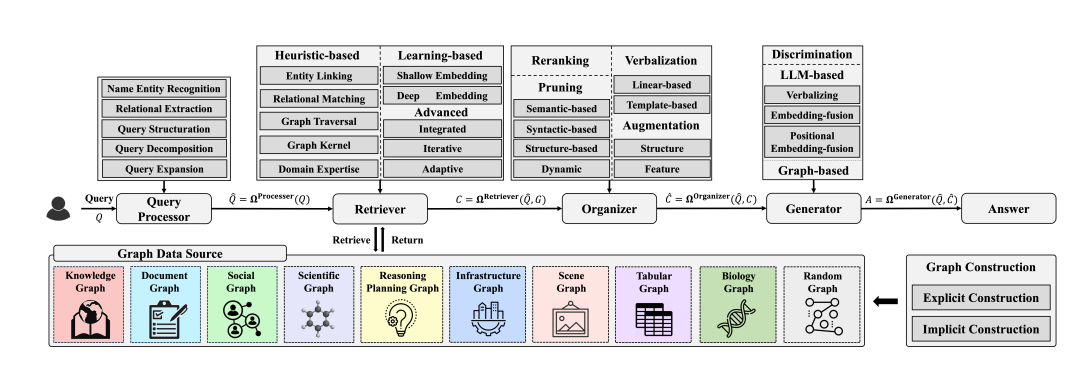
\includegraphics[width=0.98\textwidth]{images/reference-005.png}
    \caption{Kerangka umum GraphRAG dan variasi sumber graf serta komponennya (sumber: \textcite{hanRetrievalAugmentedGenerationGraphs2025})}
    \label{fig:graphrag-framework-literature}
\end{figure}

Graf dan pencarian berbasis vektor membawa kekuatan yang berbeda. Pencarian teks umumnya baik untuk menemukan bukti lokal yang serupa dengan kueri, sedangkan graf dapat membantu pertanyaan yang memerlukan hubungan eksplisit atau beberapa langkah. Edge dkk. menunjukkan pendekatan GraphRAG berbasis graf entitas dan ringkasan komunitas untuk menjawab pertanyaan global terhadap sebuah koleksi \parencite{edgeFromLocalGlobalGraph2024}. Namun, penambahan graf tidak selalu meningkatkan semua jenis pertanyaan. Nilainya bergantung pada kualitas konstruksi, resolusi identitas, strategi pencarian, dan jenis kueri.

\section{Pengelolaan Konteks Percakapan}

Sistem percakapan membawa informasi dari interaksi sebelumnya, tetapi mengirim seluruh histori
akan memperbesar konteks dan biaya \emph{token}. \emph{History compaction} merangkum histori lama,
mempertahankan fakta penting, dan menyimpan pesan terbaru. Ringkasan digunakan sebagai konteks,
sedangkan instruksi, bukti pencarian, dan memori tetap dipisahkan. Dokumen hasil pencarian
diperlakukan sebagai data, bukan instruksi, untuk mengurangi risiko \emph{indirect prompt injection}
\parencite{wuLongMemEval2025,greshakeIndirectPromptInjection2023}.

\section{Perlindungan PII}

PII adalah informasi yang dapat mengidentifikasi seseorang secara langsung atau melalui gabungan
informasi. Perlindungan dilakukan dengan mendeteksi rentang teks dan jenisnya, lalu menghapus,
mengganti, atau melakukan pseudonimisasi menggunakan pola, konteks, dan NER. Karena deteksi dapat
keliru dan PII dapat masuk ke log, artefak, indeks, atau konteks eksternal, evaluasi perlu mengukur
ketepatan deteksi serta potensi kebocoran \parencite{mccallisterGuideProtectingPII2010,
microsoftDataProtectionDeidentification2025}.

\section{\emph{Guardrail} dan Batas Kepercayaan}

\emph{Guardrail} mengizinkan, mengubah, atau menolak data pada tahap masukan dan keluaran.
Pemeriksaan berlapis diperlukan karena pesan pengguna, dokumen hasil pencarian, dan jawaban model
dapat melanggar kebijakan. Konteks eksternal diperlakukan sebagai data yang tidak tepercaya,
keluaran divalidasi, dan kegagalan pemeriksa ditangani dengan \emph{fail-closed} berupa penolakan
atau respons aman \parencite{nvidiaNeMoGuardrailsCatalog2025,liangSafeRAG2025,zouPoisonedRAG2025}.

\section{Evaluasi Sistem RAG}

Evaluasi RAG perlu memisahkan pencarian, pembentukan graf, penyusunan konteks, dan generasi.
Jawaban yang salah dapat disebabkan oleh bukti yang tidak ditemukan, konteks yang terpotong,
atau generator yang mengabaikan bukti. Karena itu, setiap tahap perlu dinilai dengan metrik yang
sesuai.

\subsection{\emph{One Factor at a Time} dan \emph{Full Factorial}}

Pada desain \emph{one factor at a time} (OFAT), satu faktor diubah sementara faktor lain dipertahankan. NIST menjelaskan bahwa pendekatan ini mudah diinterpretasikan dan cocok ketika peneliti ingin mengisolasi pengaruh suatu faktor, tetapi tidak dirancang untuk mengungkap interaksi antarfaktor \parencite{nistOneFactorAtATime}. Dalam konteks RAG, OFAT dapat menjawab pertanyaan seperti apakah mengganti \emph{chunker} meningkatkan cakupan bukti ketika indeks dan model tetap sama. Kelemahannya adalah kesimpulan hanya berlaku bersyarat pada konfigurasi yang dikunci.

Pada desain \emph{full factorial}, seluruh kombinasi level dari seluruh faktor diuji. Jika terdapat $a$, $b$, dan $c$ level pada tiga faktor, jumlah sel adalah $a\times b\times c$. Desain ini memungkinkan pengukuran pengaruh utama sekaligus interaksi, tetapi jumlah eksekusi, penyimpanan, dan biaya bertambah secara multiplikatif \parencite{nistFullFactorialDesign}. Dengan demikian, \emph{full factorial} lebih informatif untuk eksplorasi interaksi, tetapi tidak selalu proporsional dengan ruang lingkup penelitian.

Dalam praktiknya, OFAT dapat digunakan terlebih dahulu untuk menyaring kandidat atau memperoleh konfigurasi pembanding, kemudian desain faktorial digunakan ketika interaksi antarfaktor menjadi pertanyaan utama. Pemilihan urutan tersebut perlu dilaporkan secara eksplisit karena memengaruhi interpretasi hasil dan jumlah kombinasi yang diuji.

\begin{table}[H]
    \centering
    \caption{Perbandingan desain eksperimen yang relevan dengan penelitian}
    \label{tab:ofat-full-factorial}
    \small
    \renewcommand{\arraystretch}{1.35}
    \begin{tabularx}{\textwidth}{>{\RaggedRight\arraybackslash}p{0.20\textwidth} >{\RaggedRight\arraybackslash}p{0.29\textwidth} >{\RaggedRight\arraybackslash}X}
        \toprule
        \textbf{Desain} & \textbf{Karakteristik} & \textbf{Implikasi metodologis} \\
        \midrule
        \emph{OAT} & Satu faktor atau model dibandingkan dengan faktor lain dikunci. & Mudah diinterpretasikan, tetapi kesimpulannya bersifat kondisional pada faktor yang dikunci. \\
        \emph{OFAT} & Satu perubahan dibandingkan terhadap konfigurasi dasar. & Membantu mengisolasi pengaruh faktor, tetapi tidak mengukur interaksi secara menyeluruh. \\
        \emph{Full factorial} & Semua kombinasi level dari semua faktor diuji. & Memungkinkan analisis pengaruh utama dan interaksi, dengan konsekuensi jumlah eksekusi yang lebih besar. \\
        \bottomrule
    \end{tabularx}
\end{table}

\subsection{Metrik Pencarian}

Metrik pencarian harus membedakan tingkat dokumen dan tingkat unit bukti. Praktik evaluasi \emph{information retrieval} seperti BEIR juga menekankan perlunya membandingkan sistem pada himpunan pertanyaan dan relevansi yang sama \parencite{thakurBEIRHeterogeneousBenchmark2021}. \emph{Document Recall@k} menilai apakah dokumen yang memuat bukti masuk ke dalam $k$ hasil teratas, sedangkan \emph{legal-unit Recall@k} menilai apakah unit yang lebih spesifik—misalnya Pasal atau Ayat—ditemukan. Jika $Q$ adalah himpunan pertanyaan, $G(q)$ adalah himpunan dokumen atau unit emas untuk pertanyaan $q$, dan $R_k(q)$ adalah hasil teratas, maka:

\begin{equation}
    \operatorname{Recall@k}=\frac{1}{|Q|}\sum_{q\in Q}
    \mathbb{1}\left[R_k(q)\cap G(q)\neq\varnothing\right].
\end{equation}

\emph{Recall} cocok untuk menilai apakah pencari membuka jalan bagi generator. Namun, \emph{Recall} tidak menunjukkan berapa banyak hasil yang tidak relevan. Untuk menilai kemurnian hasil, \emph{Precision@k} dapat dirumuskan sebagai:

\begin{equation}
    \operatorname{Precision@k}=\frac{1}{|Q|}\sum_{q\in Q}
    \frac{|R_k(q)\cap G(q)|}{k}.
\end{equation}

Perhitungan perlu menggunakan identitas unit yang telah dideduplikasi dan tetap menggunakan penyebut $k$ ketika jumlah hasil unik lebih sedikit dari $k$. Dengan melaporkan kedua metrik pada tingkat dokumen dan unit hukum, penelitian dapat membedakan kegagalan menemukan dokumen dari kegagalan menemukan bagian normatif yang tepat.

Nilai $k$ perlu ditetapkan sebelum evaluasi dimulai karena perubahan batas tersebut dapat mengubah kesimpulan perbandingan. Pelaporan beberapa nilai $k$ membantu memperlihatkan perbedaan antara cakupan hasil yang lebih sempit dan lebih luas.

Untuk bukti yang mempunyai tingkat relevansi, \emph{nDCG} mempertimbangkan kualitas dan posisi hasil. Pada evaluasi hukum, label dapat ditetapkan sebagai 3 untuk bukti yang mendukung jawaban secara langsung, 2 untuk bukti yang diperlukan bersama bukti lain, 1 untuk konteks yang berkaitan tetapi tidak cukup sebagai dukungan, dan 0 untuk hasil yang tidak relevan. Nilai \emph{discounted cumulative gain} dan normalisasinya adalah:

\begin{equation}
    \operatorname{DCG@k}=\sum_{i=1}^{k}\frac{2^{rel_i}-1}{\log_2(i+1)},
    \qquad
    \operatorname{nDCG@k}=\frac{\operatorname{DCG@k}}{\operatorname{IDCG@k}}.
\end{equation}

MRR dapat dipakai untuk menilai posisi bukti relevan pertama, dengan $r_q$ sebagai peringkat pertama tersebut:

\begin{equation}
    \operatorname{MRR}=\frac{1}{|Q|}\sum_{q\in Q}\frac{1}{r_q},
\end{equation}

dengan kontribusi nol ketika bukti tidak ditemukan. MRR dan \emph{hit rate} berguna sebagai diagnosis, tetapi tidak menggantikan \emph{nDCG} ketika satu pertanyaan membutuhkan beberapa bukti dengan relevansi bertingkat. MAP juga tidak dijadikan metrik utama ketika anotasi emas tidak menjamin bahwa seluruh bukti relevan telah terdaftar.

\subsection{Metrik \emph{Knowledge Graph}}

Kualitas graf dapat dinilai pada tingkat relasi berarah. Sebuah relasi dianggap benar jika tripel $(source\_id,relation\_type,target\_id)$ yang dihasilkan sama dengan tripel pada anotasi emas. Metrik utama yang digunakan adalah \emph{recall}, dengan $TP$ sebagai jumlah positif benar dan $FN$ sebagai jumlah negatif salah:

\begin{equation}
    \operatorname{Recall}=\frac{TP}{TP+FN}.
\end{equation}

Metrik tersebut perlu dilengkapi validitas skema, duplikasi entitas, resolusi identitas, dan keterlacakan setiap relasi ke potongan sumber. Konfigurasi tanpa graf adalah kontrol sehingga metrik relasi untuk kondisi tersebut tidak berlaku dan harus dilaporkan sebagai N/A, bukan nol. Dampak graf pada jawaban juga perlu diukur pada pertanyaan yang memang memerlukan hubungan eksplisit, bukan digabungkan tanpa stratifikasi dengan semua pertanyaan.
